\documentclass{ltjsarticle}
%%%package読み込み
\usepackage{amsmath}
\usepackage{amssymb}
\usepackage{amsfonts}
\usepackage{mathtools}
\usepackage{bm}
% \usepackage{tikz} % ★消去: 代わりに graphicx 追加
% \usetikzlibrary{cd}
\usepackage{url}
\usepackage{graphicx} % ★追加: 図を挿入するため
\usepackage{float} % ★追加: 図の位置を制御するため
\usepackage{caption} % ★追加: 図のキャプションを柔軟に扱うため
%\usepackage{xcolor}
\usepackage{ascmac}
\usepackage{tcolorbox}
%\usepackage[dvipdfmx, setpagesize=false, bookmarks=true, bookmarksdepth=tocdepth, bookmarksnumbered=true, colorlinks=true, linkcolor=red]
\usepackage{hyperref}
\usepackage[version=4]{mhchem}
\usepackage{braket} % 追加した
\usepackage{booktabs}
\usepackage{bookmark}
%\usepackage{pxjahyper}
%%%黒板太字
\newcommand{\N}{\mathbb{N}}
\newcommand{\Z}{\mathbb{Z}}
\newcommand{\Q}{\mathbb{Q}}
\newcommand{\R}{\mathbb{R}}
\newcommand{\C}{\mathbb{C}}
\newcommand{\F}{\mathbb{F}}
%%%約物
\newcommand{\abs}[1]{\left|#1\right|}
\newcommand{\lr}[1]{\left(#1\right)}
\newcommand{\st}{\; \mathrm{s.t.}\; }
\newcommand{\Ae}{\textrm{-a.e.}} 
%%%繰り返し
\newcommand{\pluss}[3]{#1_{#2}+\cdots+#1_{#3}}
\newcommand{\minuss}[3]{#1_{#2}-\cdots-#1_{#3}}
\newcommand{\timess}[3]{#1_{#2}\times\cdots\times #1_{#3}}
\newcommand{\leqs}[3]{#1_{#2}\leq\cdots\leq #1_{#3}}
\newcommand{\geqs}[3]{#1_{#2}\geq\cdots\geq #1_{#3}}
\newcommand{\opluss}[3]{#1_{#2}\oplus\cdots\oplus #1_{#3}}
\newcommand{\otimess}[3]{#1_{#2}\otimes\cdots\otimes #1_{#3}}
\newcommand{\commas}[3]{#1_{#2},\ldots,#1_{#3}}
%%%微分
\newcommand{\dx}[1]{\mathrm{d}#1}
\newcommand{\ddx}[1]{\frac{\mathrm{d}}{\mathrm{d}#1}}
\newcommand{\dydx}[2]{\frac{\mathrm{d}#1}{\mathrm{d}#2}}
\newcommand{\dydxn}[3]{\frac{\mathrm{d}^{#3}#1}{\mathrm{d}#2^{#3}}}
\newcommand{\del}[2]{\frac{\partial#1}{\partial#2}}
\newcommand{\dell}[2]{\frac{\partial^2#1}{{\partial#2}^2}}
\newcommand{\deln}[3]{\frac{\partial^{#3}#1}{{\partial#2}^{#3}}}
%%%
%%%演算子
%log type
\let\Re\relax
\DeclareMathOperator{\Re}{Re}
\let\Im\relax
\DeclareMathOperator{\Im}{Im}
\DeclareMathOperator{\sgn}{sgn}
\DeclareMathOperator{\sign}{sign}
\DeclareMathOperator{\Supp}{Supp}
\DeclareMathOperator{\tr}{tr}
\DeclareMathOperator{\Tr}{Tr}
\DeclareMathOperator{\Det}{Det}
\DeclareMathOperator{\Log}{Log}
\DeclareMathOperator{\rank}{rank}
\DeclareMathOperator{\diag}{diag}
\DeclareMathOperator{\corank}{corank}
\DeclareMathOperator{\Res}{Res}
\DeclareMathOperator{\Ker}{Ker}
\DeclareMathOperator{\coker}{coker}
\DeclareMathOperator{\Coker}{Coker}
\DeclareMathOperator{\Var}{Var}
\DeclareMathOperator{\Cov}{Cov}
\DeclareMathOperator{\sech}{sech}
\DeclareMathOperator{\csch}{csch}
\DeclareMathOperator{\arcsec}{arcsec}
\DeclareMathOperator{\arccot}{arccot}
\DeclareMathOperator{\arccsc}{arccsc}
\DeclareMathOperator{\arccosh}{arccosh}
\DeclareMathOperator{\arcsinh}{arcsinh}
\DeclareMathOperator{\arctanh}{arctanh}
\DeclareMathOperator{\arcsech}{arcsech}
\DeclareMathOperator{\arccsch}{arccsch}
\DeclareMathOperator{\arccoth}{arccoth}
\DeclareMathOperator{\grad}{grad}
\let\div\relax
\DeclareMathOperator{\div}{div}
\DeclareMathOperator{\rot}{rot}
%\DeclareMathOperator{\GL}{GL} % ★消去 : ここから↓
%\DeclareMathOperator{\SL}{SL}
%\DeclareMathOperator{\Sym}{Sym}
%\DeclareMathOperator{\Aut}{Aut}
%\DeclareMathOperator{\Inn}{Inn}
%\DeclareMathOperator{\Out}{Out}
%\DeclareMathOperator{\id}{id}
%\DeclareMathOperator{\pr}{pr}
%\DeclareMathOperator{\supp}{supp}
%\DeclareMathOperator{\diam}{diam}
%\DeclareMathOperator{\End}{End}
%\DeclareMathOperator{\Cl}{Cl}
%\DeclareMathOperator{\Hom}{Hom} % ★消去 : ここまで↑
%limit type
\DeclareMathOperator*{\argmin}{arg~min}
\DeclareMathOperator*{\argmax}{arg~max}
%%%
%%%定理
\usepackage{amsthm}
\theoremstyle{definition}
\newtheorem{lem}{補題}
\newtheorem*{lem*}{補題}
\newtheorem{prf}{証明}
\newtheorem*{prf*}{証明}
\newtheorem*{ex*}{Example}
\newtheorem*{rem*}{Remark}
\newenvironment{prb}[1]%
{\begin{itembox}[l]{\textbf{問題 #1}}}%
{\end{itembox}}
\newenvironment{sol}[2]%
{\setcounter{lem}{0}
\setcounter{prf}{0}
\par\noindent\textbf{解答 #1} (#2)\par}%
{\par\normalfont}

\renewcommand{\refname}{Reference}


%%%%%%%%%%%%%%%%%%%%%
\numberwithin{equation}{section}
%%%%%%%%%%%%%%%%%%%%%%

\newcounter{boxeddefcounter}
\newenvironment{problem}
{\refstepcounter{boxeddefcounter}\begin{itembox}[l]{問\theboxeddefcounter}}
{\end{itembox}}

%\usepackage[hang,small,bf]{caption}
%\usepackage[subrefformat=parens]{subcaption}
\captionsetup{compatibility=false}


\newcommand{\D}{^\circ\text{C}}
\newcommand{\ka}{\textasciitilde}


\pagestyle{myheadings}
\begin{document}
\title{Organic experiment Unit.4}
\date{data: 9, 10, 14, 15, July, 2025}
\author{Author: No.7 05253011 Fumiya Kashiwai / 柏井史哉}
\maketitle
\markboth{Organic experiment Unit.4 No.7 05253011 Fumiya Kashiwai / 柏井史哉} {Organic experiment Unit.4 No.7 05253011 Fumiya Kashiwai / 柏井史哉}
%%ここまでタイトル

\newpage
\section{Purpose and background}
Hairpin rebozyme is one of the RNA enzymes that cleaves substrate RNA. To demonstrate the activity, first, we prepared template DNAs for hairpin ribozyme and substrate RNA. Then, hairpin ribozyme and substrate RNA were synthesized in vitro by transcription of template DNA. The cleavage activity was demonstrated using the RNAs. Reaction rate and the requirement for \ce{Mg^{2+}} were also examined in this experiment.

\section{Synthesis of DNA templates for hairpin ribozyme and substrate RNA}
\subsection{Experimental}
\begin{enumerate}
\item Two reaction solutions were prepared in thermal-cycler tubes (table.\ref{mix_4-2}), and mixed by pipetting gently.
\item The solutions were heated in the thermal-cycler: 95$\D$, 60 sec, then (95$\D$, 40 sec, 51$\D$, 40 sec, 72$\D$, 40 sec), 3 cycle.
\item 3 $\mu$L of each reaction solution and 3 $\mu$L of 2x DNA loading buffer were mixed and loaded in the separate wells of a 3\% agarose gel.
\item Electrophoresis was performed at 100 V for 10 min.
\item After electrophoresis, we observed the DNA products using a UV transilluminator.
\item The rest of the reaction solutions were transferred into new 600 $\mu$L tubes, and 120 $\mu$L of PCI solution was added.
\item The solutions were centrifuged at 15000$\times$g for 5 min at 25$\D$, after being mixed by pipetting and tapping.
\item The upper aqueous phase was transferred into new 600 $\mu$L tubes, and 120 $\mu$L of chloroform/isoamyl alcohol(24:1) solution was added.
\item The solutions were centrifuged at 15000$\times$g for 5 min at 25$\D$, after being mixed by pipetting and tapping.
\item The upper aqueous phase was transferred into new 600 $\mu$L tubes, and 12 $\mu$L of \ce{NaCl} solution (3 M) and 300 $\mu$L of ethanol were added.
\item The solutions were centrifuged at 15000$\times$g for 10 min at 25$\D$.
\item The supernatant was removed immediately, and 500 $\mu$L of 70\% ethanol was added.
\item The solutions were centrifuged at 15000$\times$g for 2 min at 25$\D$.
\item The supernatant was removed immediately, and the DNA pellet was dried.
\item DNA pellet was dissolved into 30 $\mu$L of ultrapure water after it completelly dried.
\end{enumerate}


\begin{table}[htp]
\caption{Reaction solutions for template DNA synthesis. "H" and "S" indicate "Hairpin ribozyme RNA" and "Substrate RNA", respectively.}
\begin{center}
\begin{tabular}{ccccc}
Reagent & concentration & H / $\mu$L & S / $\mu$L & final conc. \\ \hline\hline
Ultrapure water & - & 54 &  54 & - \\
Taq reaction buffer & 10x & 12 & 12 & 1x \\
\ce{MgCl2} aq. & 25 mM & 12 & 12 & 2.5 mM \\
dNTP solution & 5 mM each & 6 & 6 & 0.25 mM\\
forward DNA primer for H & 10 $\mu$M & 12 & 0 & 1 $\mu$M\\
reverse DNA primer for H & 10 $\mu$M & 12 & 0 & 1 $\mu$M\\
forward DNA primer for S & 10 $\mu$M & 0 & 12 & 1 $\mu$M\\
reverse DNA primer for S & 10 $\mu$M & 0 & 12 & 1 $\mu$M\\
Taq DNA polymerase & - & 12 & 12 & - \\ \hline
total &  & 120 & 120 &  
\end{tabular}
\end{center}
\label{mix_4-2}
\end{table}%

\subsection{Results and Discussion}
Template DNAs were synthesized and purified in this experiment. After the dsDNAs were synthesized by Taq polymerase, proteins (the Taq polymerase) were removed by washing with PCI and a chloroform/isoamyl alcohol (24:1) solution. Proteins denature upon exposure to phenol, becoming insoluble in both the aqueous and phenolic phases. Only DNA is soluble in the water layer, and the phenol remains in the water layer is removed by extracting with chloroform/isoamyl alcohol(24:1) solution\footnote{Question 1}. Then, DNAs were salted out using concentrated \ce{NaCl} and ethanol. DNA has a positive charge, so DNA can be salted out by adding concentrated salt such as \ce{NaCl}. The white pellet was precipitated after ethanol was added. It should be pure DNA.

%\subsection{Discussion}

%\subsection{Conclusion}
\section{Transcription of hairpin ribozyme and substrate RNA}
\subsection{Experimental}
\begin{enumerate}
\item Two reaction solutions were prepared in thermal-cycler tubes (table.\ref{mix_4-3}), and mixed by pipetting gently.
\item The reaction solutions were incubated at 37$\D$ overnight.
\item 12 $\mu$L of EDTA solution (500 mM) was added into the reaction solution and well mixed to remove the turbidity.
\item 15 $\mu$L of \ce{NaCl} solution (3 M) and 150 $\mu$L of 2-propanol were added into the reaction solution and mixed by pipetting.
\item The solutions were centrifuged at 15000$\times$g for 5 min at 25$\D$.
\item The supernatant was removed immediately, and the DNA pellet was dried.
\item The pellet was dissolved in 5 $\mu$L of ultrapure water.
\item 5 $\mu$L of 2x RNA loading buffer was added and mixed.
\item The solution for the acrylamide gel was prepared in a 15-mL tube (table.\ref{mix_gel}).
\item 75 $\mu$L of 10\% APS and 7.5 $\mu$L of TEMED were added into the gel solution and mixed.
\item The gel solution was poured into the gel plate immediately.
\item 10-well comb was put into the gel plate and left until it completely solidified.
\item The reaction solution was loaded into the acrylamide gel.
\item Urea in the well was removed by pipetting.
\item Electrophoresis was performed at 250 V for 35 min.
\item We observed the gel plate by UV after electrophoresis and excised the RNA region. 
\item The piece of the gel was transferred into a new 600-$\mu$L tube, and ground into a fine paste.
\item 500 $\mu$L of \ce{NaCl} (500 mM) / EDTA (1 mM) was added into the reaction solution and mixed, then it was shaken for 30 min using a rotisserie.
\item The gel/solution mixture was transferred to the upper unit of a filter tube and centrifuged at 8000$\times$g for 2 min at 4$\D$.
\item The solution in the bottom unit was transferred to a new 1.5-mL tube, 1 mL of ethanol was added, and mixed by pipetting.
\item The solutions were centrifuged at 15000$\times$g for 2 min at 4$\D$.
\item The supernatant was removed immediately, and 1 mL of 70\% ethanol was added.
\item The solutions were centrifuged at 15000$\times$g for 2 min at 4$\D$.
\item The supernatant was removed immediately, and the DNA pellet was dried.
\item The pellet was dissolved in 10 $\mu$L of ultrapure wate after it completelly dried.
\item The UV absorption of the two samples was measured.
\item The two solutions were diluted by ultrapure water into 10 $\mu$M (Hairpin) and 50 $\mu$L (Substrate) solutions.
\end{enumerate}

\begin{table}[htp]
\caption{Reaction solutions for RNA synthesis. "H" and "S" indicate "Hairpin ribozyme RNA" and "Substrate RNA", respectively.}
\begin{center}
\begin{tabular}{ccccc}
Reagent & concentration & H / $\mu$L & S / $\mu$L & final conc. \\ \hline\hline
Ultrapure water & - & 31.5 & 31.5 & - \\
T7 buffer & - & 19.5 & 19.5 & -  \\
DTT & 100 mM & 15 & 15 & - \\
\ce{MgCl2} aq. & 250 mM & 18 & 18 & 30 mM \\
NTP solution & 25 mM each & 30 & 30 & 5 mM\\
DNA template for H & - & 30 & 0 & - \\
DNA template for S & - & 0 & 30 &  - \\
Taq DNA polymerase & - & 6 & 6 & - \\ \hline
total &  & 150 & 150 &  
\end{tabular}
\end{center}
\label{mix_4-3}
\end{table}%

\begin{table}[htp]
\caption{Reaction solutions for RNA synthesis. "H" and "S" indicate "Hairpin ribozyme RNA" and "Substrate RNA", respectively.}
\begin{center}
\begin{tabular}{ccccc}
Reagent & concentration & volume & final conc. \\ \hline\hline
acrylamide/bisacrylamide (19:1) & 40\% & 3 mL & 15\%\\ 
TBE buffer & 5x & 1.6 mL & 1x \\
Urea & - & 3.36 g & - \\
Ultrapure water & - & up to 8 mL & -\\ \hline
total & - & 8 mL & - 
\end{tabular}
\end{center}
\label{mix_gel}
\end{table}%



\subsection{Resalts and Discussion}
After the transcription reaction was performed overnight, the reaction solution was turbid. As the turbidity was removed by adding EDTA solution, the turbidity was thought to be caused by \ce{Mg^{2+}} ion. This suggests that the turbidity was an aggregation of RNA and proteins.\footnote{Question 2}

For the electrophoresis gels of RNA, we used urea. Urea is needed because it weakens the hydrogen bond within RNA and keeps the RNA straight chain formation. Urea weakens the hydrogen bond within RNA because it is highly polarized and can form hydrogen bonds with RNA. 
RNA favors complex secondary structure, but in a complex structure, it is difficult to separate them by length in electrophoresis\footnote{Question 3}.
 
In the preparation of PAGE gel, APS and TEMED work as radical initiators. First, the \ce{O-O} bond in APS cleaves (shown in fig.\ref{APS}), and TEMED becomes a stable radical. The TEMED radical attacks the acrylamide and works as a radical initiator\footnote{Question 4}.

The result of the UV absorption measurement was shown in fig.\ref{fig_nanodrop} and table.\ref{table_nanodrop}. The concentration of each sample was calculated by assuming that the absorbance at 260 nm (A260) is proportional to the concentration of the RNA sample, and A260 = 1 is equivalent to 40 ng/$\mu$L.  Also, the absorbance at 280 nm was recorded as A280, and A260/A280 was calculated as an index of the purity of the RNA samples. According to \cite{thermo}, pure RNA typically has an A260/A280 of 2.0, and a small change (0.2-0.3) occurs by pH change. The A260/A280 values of our samples indicated that they are pure RNA samples.

\begin{figure}[htbp]
\begin{center}
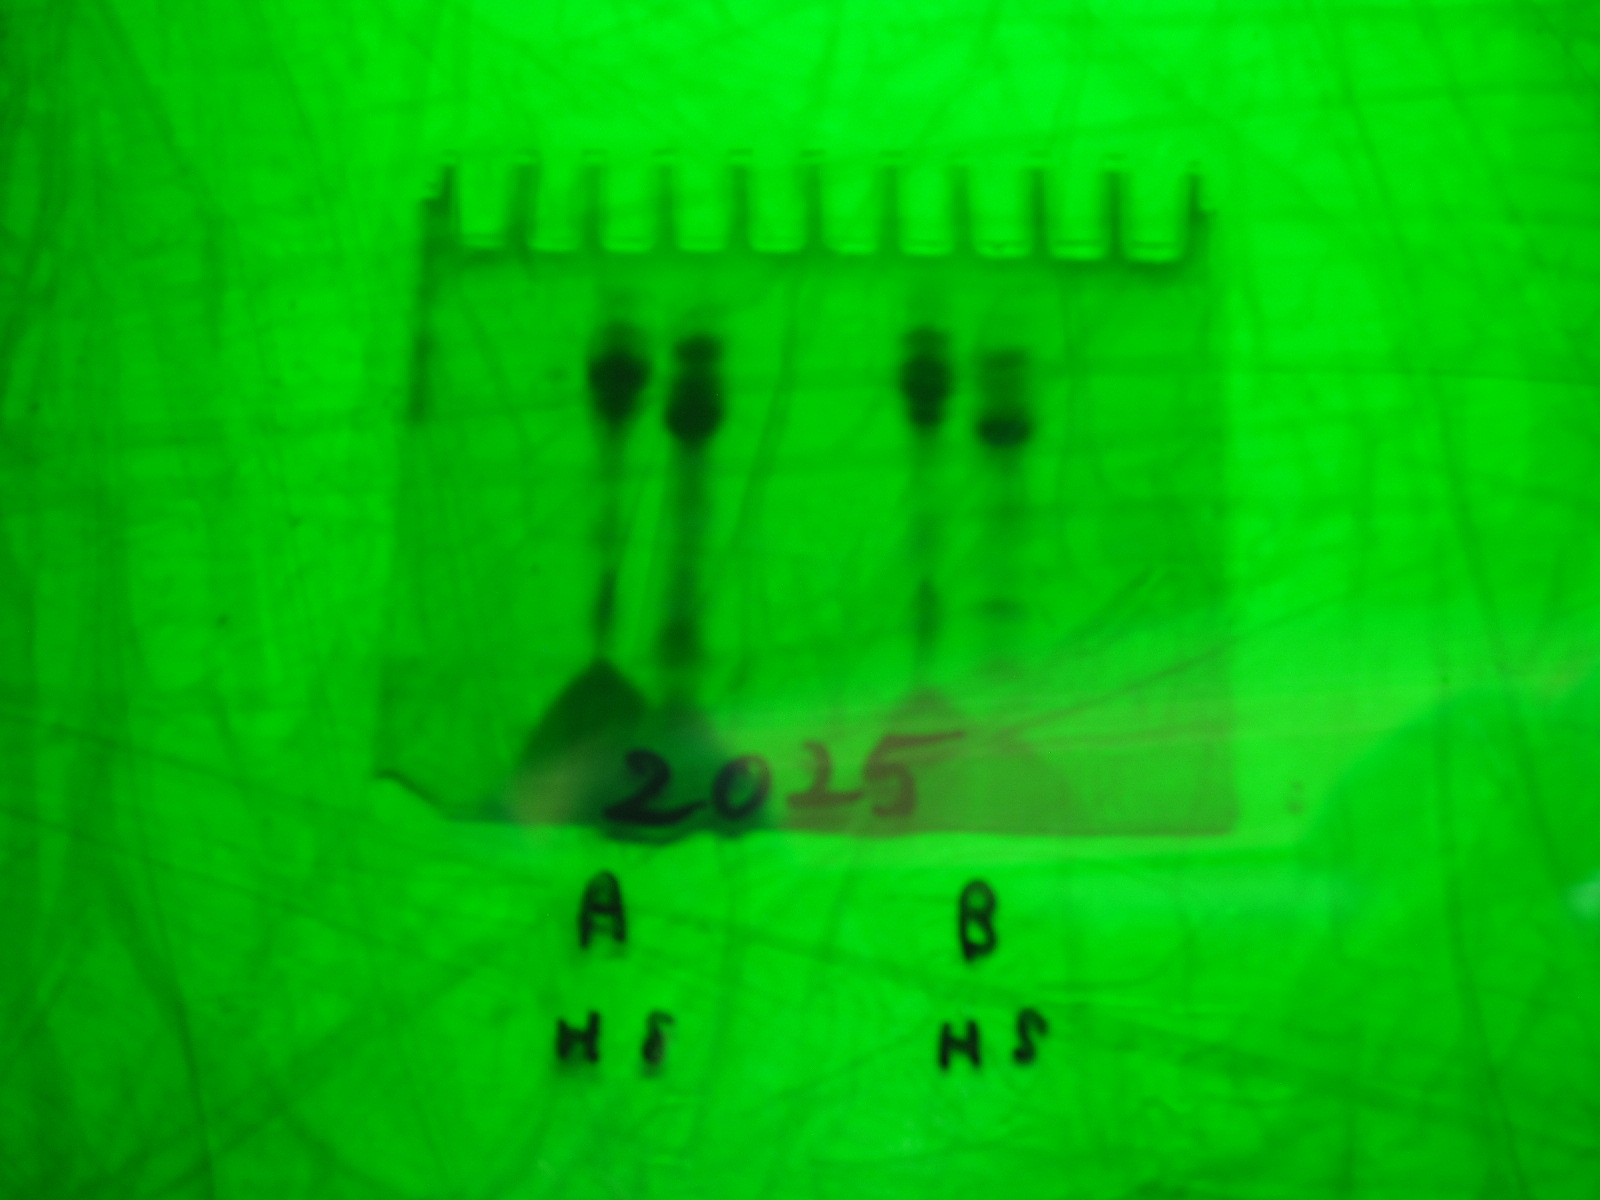
\includegraphics[width = 10 cm]{250711_A,B.JPG}
\caption{Agalose gel after the electrophoresis in sec 3.2. The right side (B), our sample Hairpin / Substrate were shown.}
\label{gel}
\end{center}
\end{figure}

\begin{table}[htp]
\caption{UV absorbance values of refined RNA samples and calculated concentration of each sample}
\begin{center}
\begin{tabular}{cccccc}
\hline
 & A260 & A280 & A260/A280 & Mw / kDa & conc. / $\mu$M \\ \hline\hline
Hairpin & 43.947 & 19.632 & 2.24 & 17.24 & 102\\
Substrate & 21.925 & 11.259 & 1.95 & 11.85& 74.0 \\\hline
\end{tabular}
\end{center}
\label{table_nanodrop}
\end{table}%

\begin{figure}[htbp]
 \begin{minipage}[b]{0.5\linewidth}
  \centering
  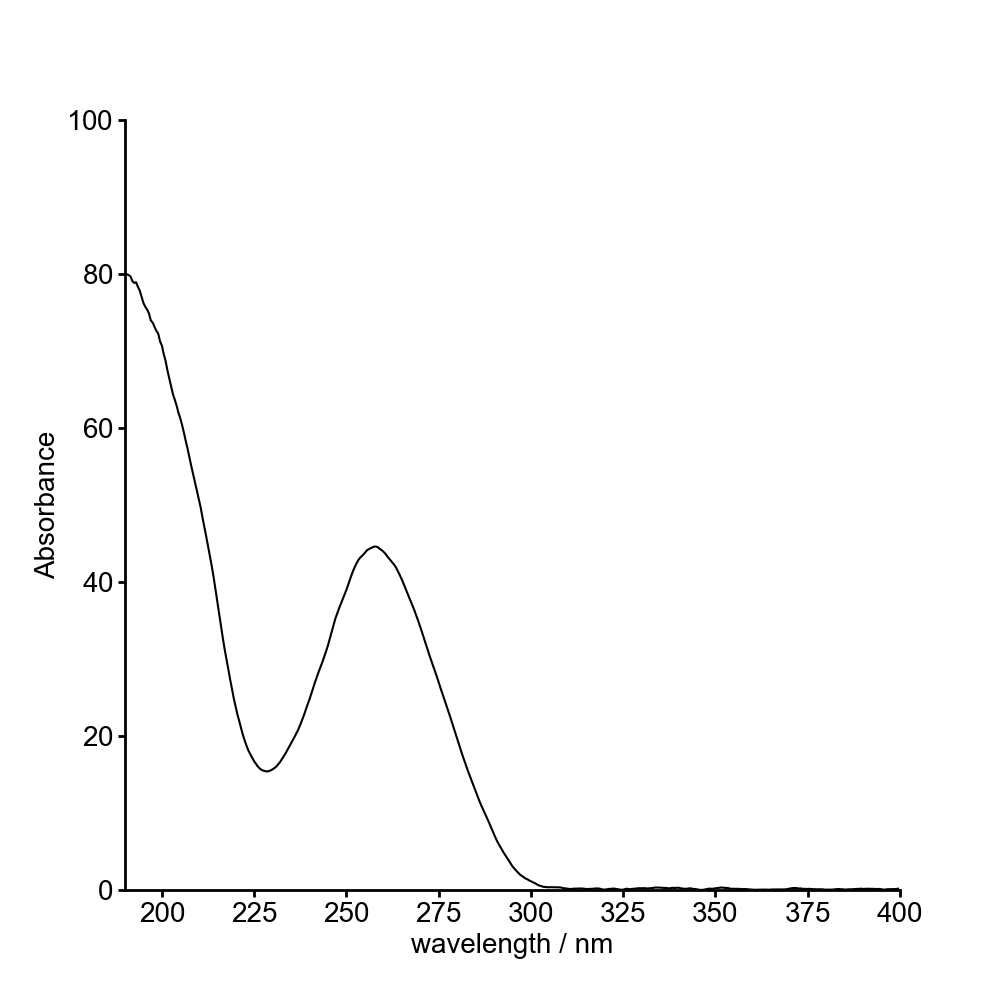
\includegraphics[keepaspectratio, scale=0.3]
  {B_Hairpin_UV-vis.png}
  \subcaption{Hairpin RNA}
 \end{minipage}
 \begin{minipage}[b]{0.5\linewidth}
  \centering
  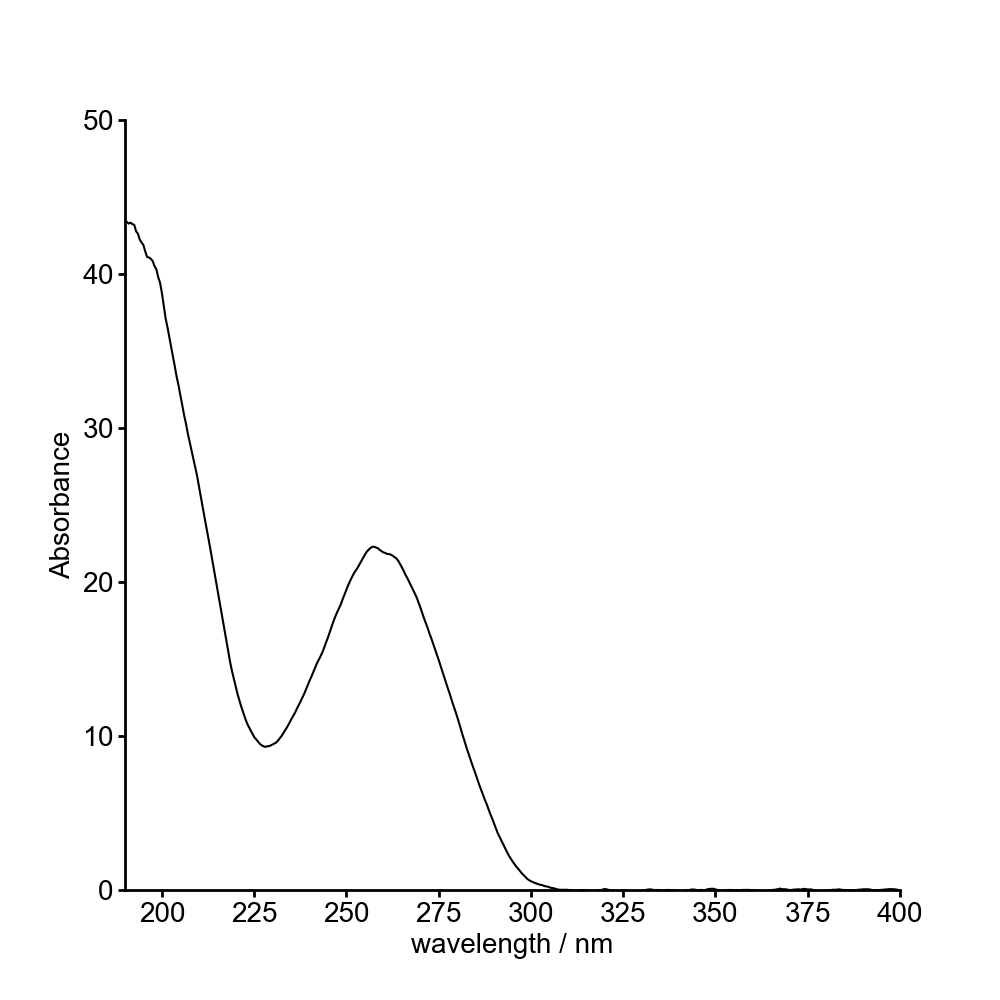
\includegraphics[keepaspectratio, scale=0.3]
  {B_Substrate_UV-vis.png}
  \subcaption{Substrate RNA}
 \end{minipage}
 \caption{UV-Vis spectrum of hairpin RNA and substrate RNA}
 \label{fig_nanodrop}
\end{figure}

\begin{figure}[htbp]
\begin{center}
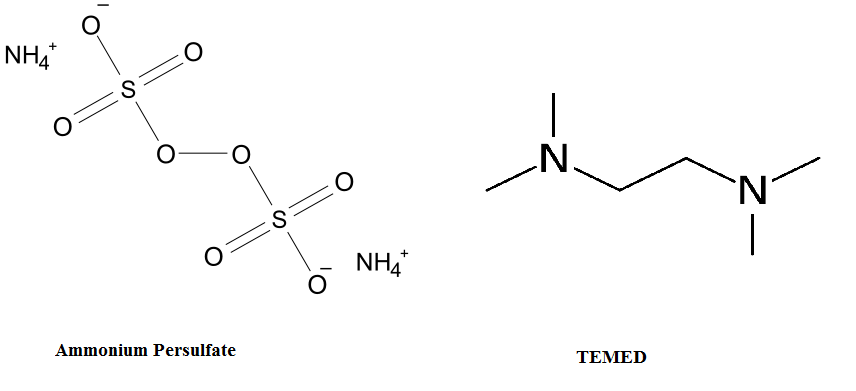
\includegraphics[width = 10 cm]{structure.png}
\caption{The structures of APS and TEMED}
\label{APS}
\end{center}
\end{figure}


\newpage
\section{Cleavage of substrate RNA by hairpin robozyme}
\subsection{Experimental}
\begin{enumerate}
\item Reaction solutions (A-F) in a 600-mL tube (table.\ref{mix_4-4}).
\item The reaction solutions were incubated at 95$\D$ for 2 min. 
\item \ce{MgCl2} solution (50 mM) or ultrapure water was added to the reaction solutions.
\item The reaction solutions were incubated at 37$\D$ for several minutes (written in table.\ref{mix_4-4}).
\item 10 $\mu$L of RNA 2x loading buffer was added after the incubation.
\item An acrylamide gel was prepared in the same manner as 4-3.
\item 10 $\mu$L of each sample was loaded into the well of the gel plate.
\item Electrophoresis was performed at 250 V for 40 min.
\item The gel was strained by incubating in ethidium bromide solution (0.5 $\mu$g/mL) for 10 min.
\item We observed the gel plate under UV.
\end{enumerate}

\begin{table}[htp]
\caption{Reaction solutions for cleavage of substrate RNA}
\begin{center}
\begin{tabular}{ccccccccc}
Reagent & concentration & A / $\mu$L & B / $\mu$L & C / $\mu$L & D / $\mu$L & E / $\mu$L & F / $\mu$L & final conc. \\ \hline\hline
Ultrapure water & - & 2 &  2 & 2 & 2 & 2 & 2 & - \\
Tris-HCl (pH 7.5) & 100 mM & 4 & 4 & 4 & 4 & 4 & 4 & 40 mM \\
hairpin ribozyme & 10 $\mu$M & 2 & 0 & 2 & 2 & 2 & 2 & 2 $\mu$M\\
substrate RNA & 50 $\mu$M & 0 & 2 & 2 & 2 & 2 & 2 & 10 $\mu$M \\ \hline 
\ce{MgCl2} aq. & 50 mM & 2 & 2 & 2 & 2 & 2 & 0 & 10 mM \\ 
ultrapure water & - & 0 & 0 & 0 & 0 & 0 & 2 & - \\ \hline
total & - & 10 & 10 & 10 & 10 & 10 & 10 & -  \\ \hline \hline
incubated time & - & 30 min & 30 min & 0 min & 5 min & 30 min & 30 min & - \\
\end{tabular} 
\end{center} 
\label{mix_4-4} 
\end{table}% 


\subsection{Resalts and Discussion}
By mistake, we put the reaction tube in the wrong place in the heat block, and the first 5 minutes of incubation were insufficient. So, solution D is not incubated sufficiently. We prepared another solution D' and incubated it for 5 minutes. Other samples were incubated for 30 minutes after we noticed the problem and moved them to the right heat block. 

The result of electrophoresis after incubation is shown in fig.\ref{incubation}. 4 major bands were observed.
Band 1 and 2 is attributed to the Hairpin RNA and substrate RNA, respectively. And bands 3 and 4 show the existence of shorter 2 RNAs than the substrate RNA, which are attributed to the cleaved RNAs. In addition to that, when bands 3 and 4 appear, band 2 is thinner, suggesting that bands 3 and 4 are the cleaved RNA of the substrate RNA.
In this experiment, samples D, D', and E showed the cleaved products. This result shows that the cleavage reaction of substrate RNA occurs only in the presence of the Hairpin RNA and \ce{Mg^{2+}}.

In addition to that, only incubation for 5 min (even the heating is insufficient), the cleavage reaction occurs. On the other hand, even after a 30-minute reaction, in sample E, band 2 remains, suggesting the cleavage reaction is not finished.

\begin{figure}[htbp]
\begin{center}
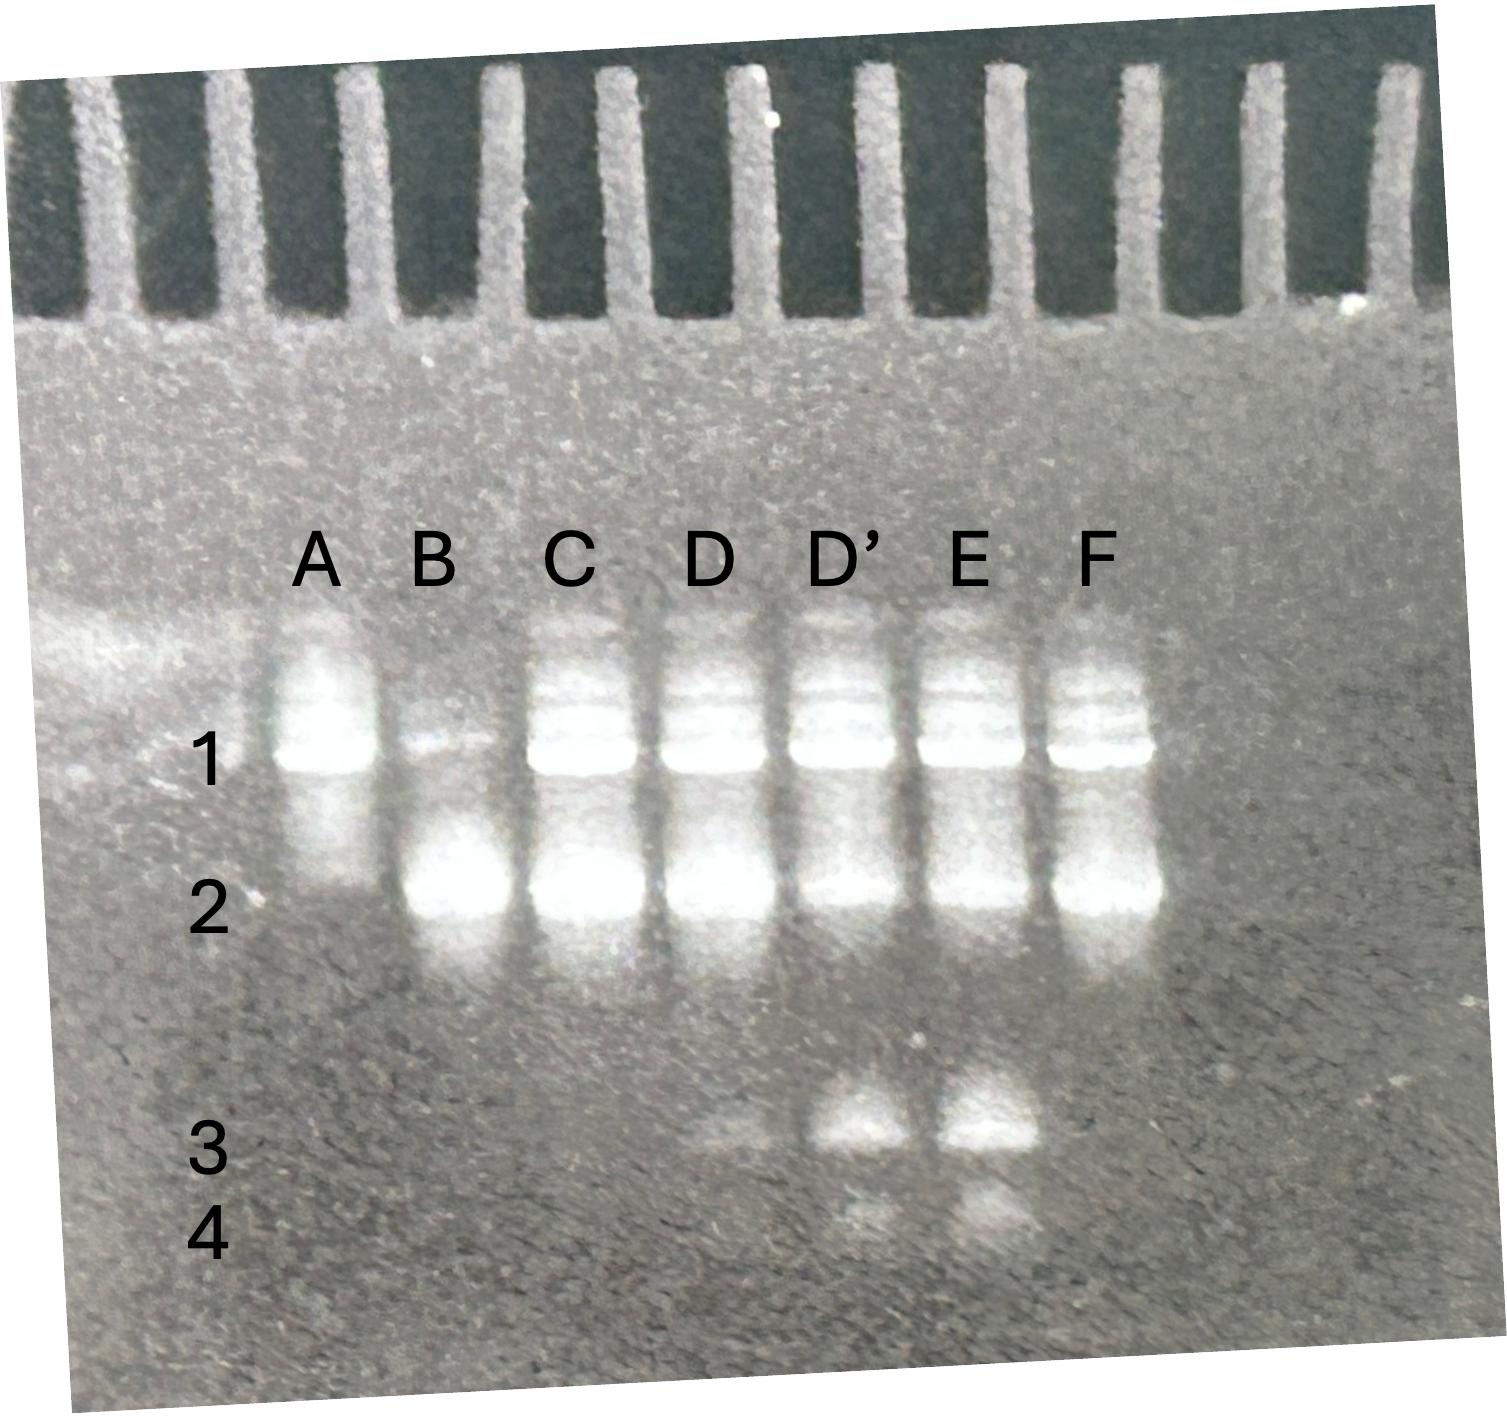
\includegraphics[width = 10 cm]{incubation.png}
\caption{PAGE gel picture after incubation}
\label{incubation}
\end{center}
\end{figure}

The reaction mechanism proposed for the cleavage reaction is shown in fig.\ref{mechanism} \cite{mechanism}. According to \cite{mechanism}, \ce{Mg^{2+}} itself does not involve the hydrolysis, only stabilizes the transition formation, and this is unique to hairpin rebozyme. And the cleavage reaction can be considered an acid/base reaction. Ribozyme is considered to work as an acid and base in hydrolysis. Generating the favorable confirmation for the reaction by hybrization is also considered to be important for the activation of the reaction\footnote{Question 5}.

\begin{figure}[htbp]
\begin{center}
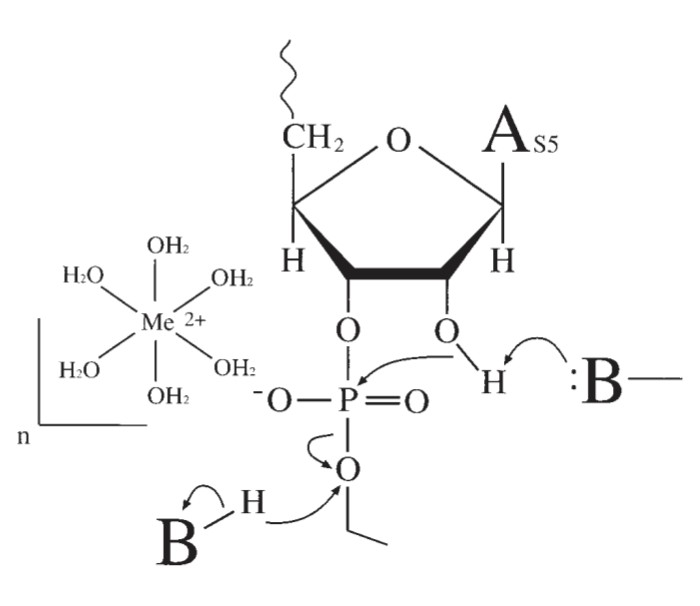
\includegraphics[width = 10cm]{mechanism.png}
\caption{proposed reaction mechanism of cleaved reaction. }
\label{mechanism}
\end{center}
\end{figure}


%\newpage
%\section{Appendix}





%%参考文献
\begin{thebibliography}{99}
\bibitem{thermo}
Thermo Fisher Scientific - NanoDrop products, 
\url{https://dna.uga.edu/wp-content/uploads/sites/51/2019/02/Note-on-the-260_280-and-260_230-Ratios.pdf}
\bibitem{structure}
What are the uses of APS and TEMED in SDS PAGE protocol? - InfoBiochem
\url{https://www.infobiochem.com/uses-of-aps-and-temed-in-sds-page-protocol/}
\bibitem{mechanism}
Shippy, Richard and Lockner, Randy and Farnsworth, Margaret and Hampel, Arnold, The hairpin ribozyme, Molecular Biotechnology, 1999(12). 1. 117-129.


\end{thebibliography}

\end{document}